\section{Auswertung}
\label{sec:Auswertung}
Jegliche Fehlerrechnung wurde mit der python-Bibliothek uncertainties \cite{uncertainties} absolviert.
Trotz dessen sind die Formeln für die Unsicherheiten in den jeweiligen Abschnitten angegeben.
Allgemeine Rechnungen wurden mit der python-Bibliothek numpy \cite{numpy} automatisiert. 
Die graphischen Untersützungen wurden mit Hilfe der python-Bibliothek matplotlib \cite{matplotlib} erstellt.
\subsection{Bestimmung der Untergrundrate}
Zu der Messung der Untergrundrate wurde ein Zeitintervall von $\symup{\Delta} t = \SI{300}{\second}$ gewählt.
Ingesamt ergaben sieben Messungen die Werte:
\begin{equation*}
    N_U = \{ 129, 143, 144, 136, 139, 126, 158 \}
\end{equation*}
Der Mittelwert der Untergrundrate beträgt
\begin{equation*}
    \bar{U}_N = 139.2857
\end{equation*}
\subsection{Bestimmung der Halbwertszeit von Vanadium}
\label{sub:Vana}
Bevor die Messdaten ausgewertet werden können, muss der Mittelwert der Hintergrundrate mit dem Zeitintervall von $\symup{\Delta} t = \SI{30}{\second}$
abgezogen werden. Dieser beträgt
\begin{equation*}
    \bar{U}_\text{N, \SI{30}{\second}} = 13.9286 \approx 14 \; \text{.}
\end{equation*}
Die Dezimalstellen des Mittelwerts wurden durch Runden eleminiert, da es nur ganze Vanadium-Kerne geben kann.
In der Tabelle \ref{tab:vana} sind die instabilen Vanadium-Kerne ohne Abzug der Untergrundrate $\tilde{N}$ und die instabilen Vanadium-Kerne mit Abzug 
der Untergrundrate aufgetragen.
\begin{table}
    \centering
    \caption{Instabile Vanadium-Kerne}
    \label{tab:vana}
    \begin{tabular}{S[table-format=3.0] S[table-format=3.0] S[table-format = 3.0] @{${}\pm{}$} S[table-format = 1.2]
                    S[table-format=4.0] S[table-format=2.0] S[table-format = 2.0] @{${}\pm{}$} S[table-format = 1.2]}
        \toprule
        {$t \mathbin{/} \si{\second}$} & {$\tilde{N}$} & \multicolumn{2}{c} {$N$} & {$t \mathbin{/} \si{\second}$} & {$\tilde{N}$} & \multicolumn{2}{c} {$N$} \\
        \midrule
        30	&    189    & 175 & 1.32 & 690  &  35  & 21  & 4.58    \\
        60	&    197    & 183 & 1.35 & 720  &  19  & 50  & 2.23    \\
        90	&    150    & 136 & 1.16 & 750  &  28  & 14  & 3.74    \\
        120	&    159    & 145 & 1.20 & 780  &  27  & 13  & 3.60    \\
        150	&    155    & 141 & 1.18 & 810  &  36  & 22  & 4.69    \\
        180	&    132    & 118 & 1.08 & 840  &  25  & 11  & 3.31    \\
        210 &	 117    & 103 & 1.01 & 870  &  29  & 15  & 3.87    \\
        240 &	 107    & 93  & 9.64 & 900  &  18  & 40  & 2.00    \\
        270 &	 94     & 80  & 8.94 & 930  &  17  & 30  & 1.73    \\
        300 &	 100    & 86  & 9.27 & 960  &  24  & 10  & 3.16    \\
        330 &	 79     & 65  & 8.06 & 990  &  21  & 70  & 2.64    \\
        360 &	  69    & 55  & 7.41 & 1020 &  25  & 11  & 3.31    \\
        390 &	  81    & 67  & 8.18 & 1050 &  21  & 70  & 2.64    \\
        420 &	  46    & 32  & 5.65 & 1080 &  24  & 10  & 3.16    \\
        450 &	  49    & 35  & 5.91 & 1110 &  25  & 11  & 3.31    \\
        480 &	  61    & 47  & 6.85 & 1140 &  17  & 30  & 1.73    \\
        510 &	  56    & 42  & 6.48 & 1170 &  20  & 60  & 2.44    \\
        540 &	  40    & 26  & 5.09 & 1200 &  19  & 50  & 2.23    \\
        570 &	  45    & 31  & 5.56 & 1230 &  20  & 60  & 2.44    \\
        600 &	  32    & 18  & 4.24 & 1260 &  18  & 40  & 2.00    \\
        630 &	  27    & 13  & 3.60 & 1290 &  16  & 20  & 1.41    \\
        660 &	  43    & 29  & 5.38 & 1320 &  17  & 30  & 1.73    \\
    \bottomrule     
    \end{tabular}
\end{table}
Zu der Bestimmung der Halbwertszeit wird das Zerfallsgesetz $REFERENZ$ logarithmiert, so dass sich die Umformung
\begin{equation}
\ln \left (\frac{N}{N_0} \right ) = - \lambda t 
\end{equation}
Somit lässt sich eine lineare Ausgleichrechung mit der Geradengleichung
\begin{equation}
    y = at + b 
\end{equation}
durchführen. 
Für Regressionsparameter $a$ n und $b$ ergibt sich
\begin{align*}
    a &= \SI{-0.0032(2)}{\per\second} = - \lambda\\
    b &= \num{0.0213(1275)}
\end{align*}
\begin{figure}
    \centering
    \caption{Zerfallskurve von Vanadium}
    \label{fig:vana}
    \includegraphics{build/vana.pdf}
\end{figure}
Mit Hilfe der Gleichung $REFERENZ$ lässt sich die Halbwertszeit zu
\begin{equation*}
\tau = \SI{219(11)}{\second}
\end{equation*}
bestimmen.
Der Fehler der übrigen Kerne lässt sich mittels
\begin{equation}
    \symup{\Delta} N = \sqrt{N} 
\end{equation}
errechnen.
Nach der Gaußschen Fehlerfortpflanzung wird die Unsicherheit der Halbwertszeit durch
\begin{equation}
    \symup{\Delta} \tau = \frac{\ln \left (2 \right )}{\lambda^2} \symup{\Delta} \lambda
\end{equation}
\subsection{Bestimmung der Halbwertszeit von Rhodium}
Wie bereits in Abschnitt \ref{sub:Vana} muss der Mittelwert der Hintergrundrate abgezogen werden.
Da die übrigen Rhodium-Kerne mit einem Intervall von $\symup{\Delta} = \SI{15}{\second}$ gemessen wurden, muss der Mittelwert der Untergrundrate
auf dieses Zeitintervall herunterskaliert werden.
\begin{equation*}
    \bar{U}_\text{N, \SI{15}{\second}} = 6.9644 \approx 7 \; \text{.}
\end{equation*}
Wie bereits in Abschnitt \ref{sub:Vana} wurden die  Dezimalstellen des Mittelwert Runden eleminiert (selbige Begründung).
In der Tabelle \ref{tab:vana} sind die instabilen Rhodium-Kerne ohne Abzug der Untergrundrate $\tilde{N}$ und die instabilen Rhodium-Kerne mit Abzug 
der Untergrundrate aufgetragen.
%\begin{table}
%    \centering
%    \caption{Instabile Vanadium-Kerne}
%    \label{tab:vana}
%    \begin{tabular}{S[table-format=3.0] S[table-format=3.0] S[table-format = 3.0] @{${}\pm{}$} S[table-format = 1.2]
%                    S[table-format=4.0] S[table-format=2.0] S[table-format = 2.0] @{${}\pm{}$} S[table-format = 1.2]}
%        \toprule
%        {$t \mathbin{/} \si{\second}$} & {$\tilde{N}$} & \multicolumn{2}{c} {$N$} & {$t \mathbin{/} \si{\second}$} & {$\tilde{N}$} & \multicolumn{2}{c} {$N$} \\
%        \midrule
%        15  &  667
%        30  &  585
%        45  &  474
%        60  &  399
%        75  &  304
%        90  &  253
%        105 &  213
%        120 &  173
%        135 &  152
%        150 &  126
%        165 &  111
%        180 &   92
%        195 &   79
%        210 &   74
%        225 &   60
%        240 &   52
%        255 &   56
%        270 &   53
%        285 &   41
%        300 &   36
%        315 &   37
%        330 &   32
%        \bottomrule     
%    \end{tabular}
%\end{table}
\begin{figure}
    \centering
    \caption{Zerfallskurve von Rhodium}
    \label{fig:rho}
    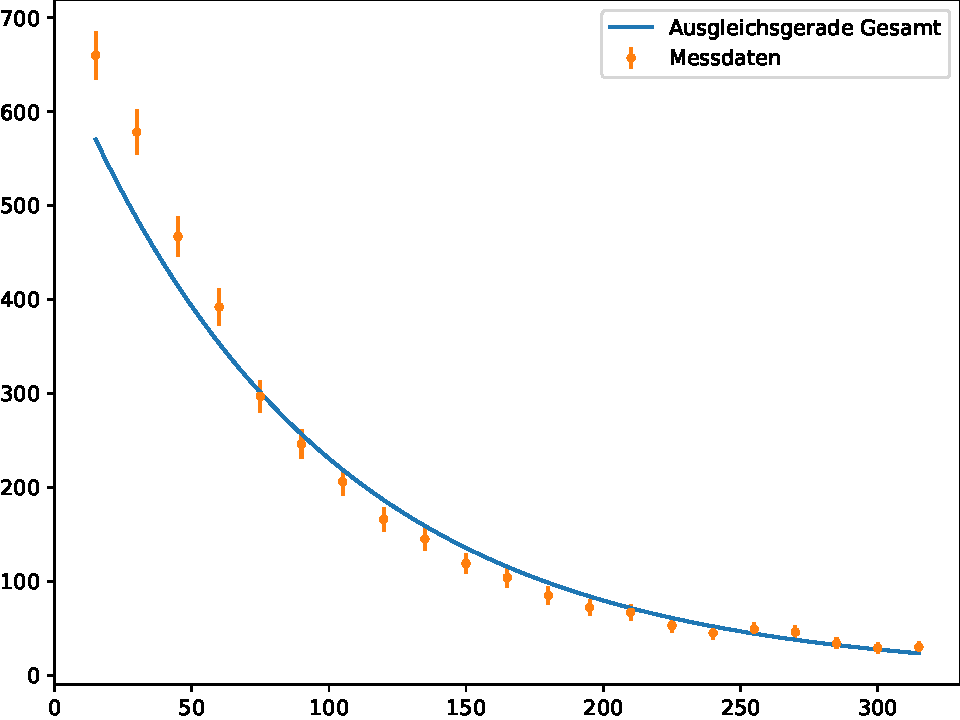
\includegraphics{build/rho.pdf}
\end{figure}